\documentclass[12pt]{article}

\usepackage[spanish]{babel}
\usepackage[utf8x]{inputenc}
\usepackage{amsmath}

\usepackage{hyperref}
\usepackage{url}
\usepackage{gensymb}
\usepackage[dvipsnames]{xcolor}

\usepackage{parskip}
\usepackage{fancyhdr}
\usepackage{multicol}
\usepackage{vmargin}
\usepackage{setspace}
\usepackage{geometry}

\usepackage{float}
\usepackage{array}
\usepackage{graphicx}
\graphicspath{{images/}}
\usepackage{wrapfig}
\usepackage{caption}
\usepackage{subcaption}

\setmarginsrb{2 cm}{1 cm}{2 cm}{1.5 cm}{1 cm}{1 cm}{1 cm}{1 cm}

\title{ Medición de variación de temperatura}
\author{Martín Alejandro Paredes Sosa}		

\makeatletter
\let\thetitle\@title
\let\theauthor\@author
\let\thedate\@date										
\makeatother

\pagestyle{fancy}
\fancyhf{}
\rhead{Lic.. Física}
\lhead{Informe 2:\thetitle}
\cfoot{\thepage}

\begin{document}
%%%%%%%%%%%%%%%%%%%%%%%%%%%%%%%%%%%%%%%%%%%%%%%%%%%%%%%%%%%%%%%%%%%%%%%%%%%%%%%%%%%%%%%%
%\begin{titlepage}
%	\centering
%    \vspace*{0.5 cm}
%    
\includegraphics[scale = 0.5]{logo}\\[0.5 cm]	% University Logo
%    \textsc{\LARGE Universidad de Sonora}\\[1 cm]	% University Name
%	\textsc{\Large División de Ciencias Exactas y Naturales}\\[1 cm]		%		% Course Code
%	\textsc{\large Termodinámica Clásica}\\[0.5 cm]				% Course Name
%	\rule{\linewidth}{0.2 mm} \\[0.4 cm]
\begin{center}
{ \large \bfseries \thetitle}\\
\end{center}
%{ \large \bfseries \thetitle}\\
%	\rule{\linewidth}{0.2 mm} \\[1.25 cm]
%    \textsc{\Large Equipo \#2} \\[1.25 cm]
%\thetitle\\	
	\begin{minipage}{\textwidth}
		\begin{center} 
			%\textsc{\Large Integrantes:} \large \\
			\theauthor 
			\end{center}
	\end{minipage}\\[0.2 cm]
%	\vfill
	
%\end{titlepage}
%===================================================================================================
%\pagebreak
%\tableofcontents
%\pagebreak
%===================================================================================================
\begin{abstract}
	Esta practica consistió en medir la variación de la temperatura de tres diferentes calorímetros (diferentes materiales). La segunda medición de temperatura se realizó con otros 3 contenedores del mismo material pero con una superficie exterior de diferente color.
\end{abstract}
\vspace{-1cm}
%===================================================================================================
\section{Introducción}
\vspace{-.5cm}
En está práctica se realizaron mediciones de temperatura para calorímetros de diferentes materiales. El objetivo de esto era observar si el tipo de contenedor, en nuestro caso los calorímetros, afectan como la varia la temperatura conforme pasaba el tiempo. Lo que se espera es saber cual de los calorímetros mantiene mejor la temperatura.

\hspace{0.5cm} La segunda parte consistió en observar la variación de la temperatura para contenedores de un mismo material y grosor pero con un exterior de diferente color (en nuestro caso se pintaron con pintura blanca y negro en aerosol). El objetivo de este otro experimento es ver si tiene algún efecto esta diferencia en la forma que varia la temperatura.

%El objetivo de los experimentos es medir la variación de la temperatura con el tiempo para evaluar características de las fronteras.
\vspace{-.75cm}
%===================================================================================================
\section{Desarrollo Experimental}
\vspace{-.5cm}
La práctica consistió en dos experimentos cuantitativos donde se realizaron mediciones temperatura de agua caliente en diferentes contenedores. El primer experimento fue el siguiente:
\vspace{-1.cm}
\subsection{Variación en calorímetros}
\vspace{-.25cm}
Se tomaron tres recipientes conocidos como calorímetros. Uno de los calorímetros era de unicel, otro era de metal y el ultimo era de exterior de metal e interior de unicel. A estos recipientes se les introdujo agua caliente a 80°C para tener así las mismas condiciones. Se taparon dichos contenedores y se les coloco un termómetro \textit{Quad Temperature Sensor} con cuatro sondas de temperatura de respuesta rápida en cada unos de los calorímetros. El cuarto sensor se introdujo en un recipiente con agua que se había dejado reposar desde antes para medir la temperatura ambiente. El \textit{Quad Temperature Sensor} tiene un rango de -35 a 135°C con una exactitud de $\pm 0.5$°C y una resolución de 0.0025°C  con una sonda de respuesta rápida con rango de -10°C a 70°C.\\

\begin{figure}[H]
\centering
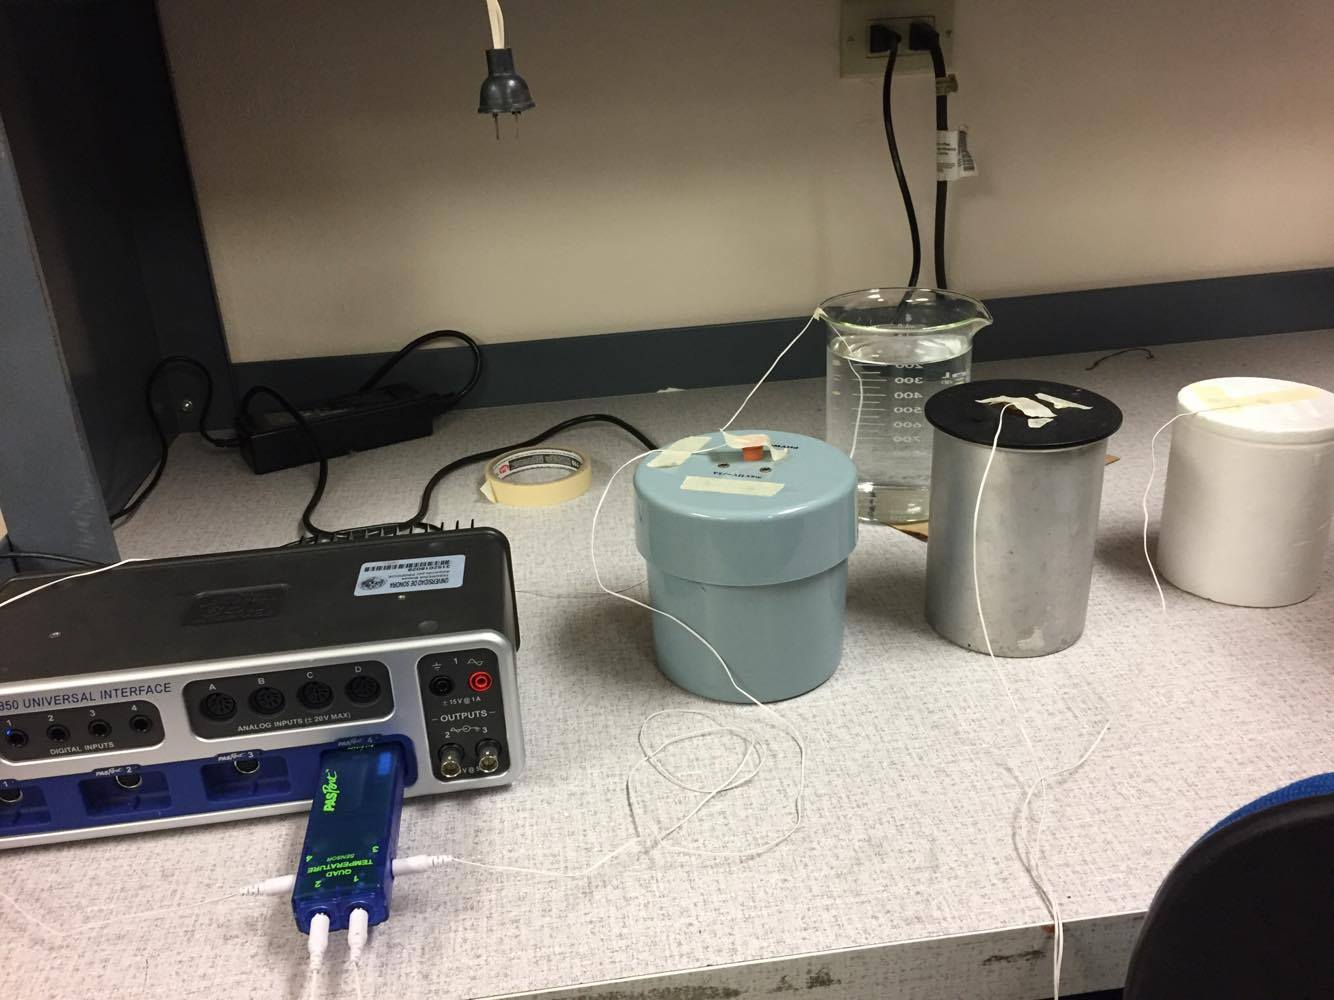
\includegraphics[height=5cm]{calorimetro.jpg}
\caption{Arreglo del experimento con los calorímetros }
\end{figure}

\hspace*{0.5cm} Se conecto el termómetro a la interfaz y se ajusto la frecuencia de muestreo a 30 segundos. El experimento duro 30 minutos.

%\vspace{0.5cm} 
El segundo experimento fue utilizando otros tres recipientes metálicos en los cuales  se midió como varia la temperatura mientra transcurría el tiempo.
\vspace{-0.5cm} 
\subsection{Variación en recipientes metálicos}
Se tomaron los tres recipientes y se llenaron con agua caliente a 78°C para tener las misma condiciones. A estos recipientes se taparon y se les inserto un termómetro \textit{Temperature-Sensor PS-2125}. Este tiene un rango de -35 a 135°C, una exactitud de $\pm 0.5$°C y una resolución de 0.01°C. 

\begin{figure}[H]
\centering
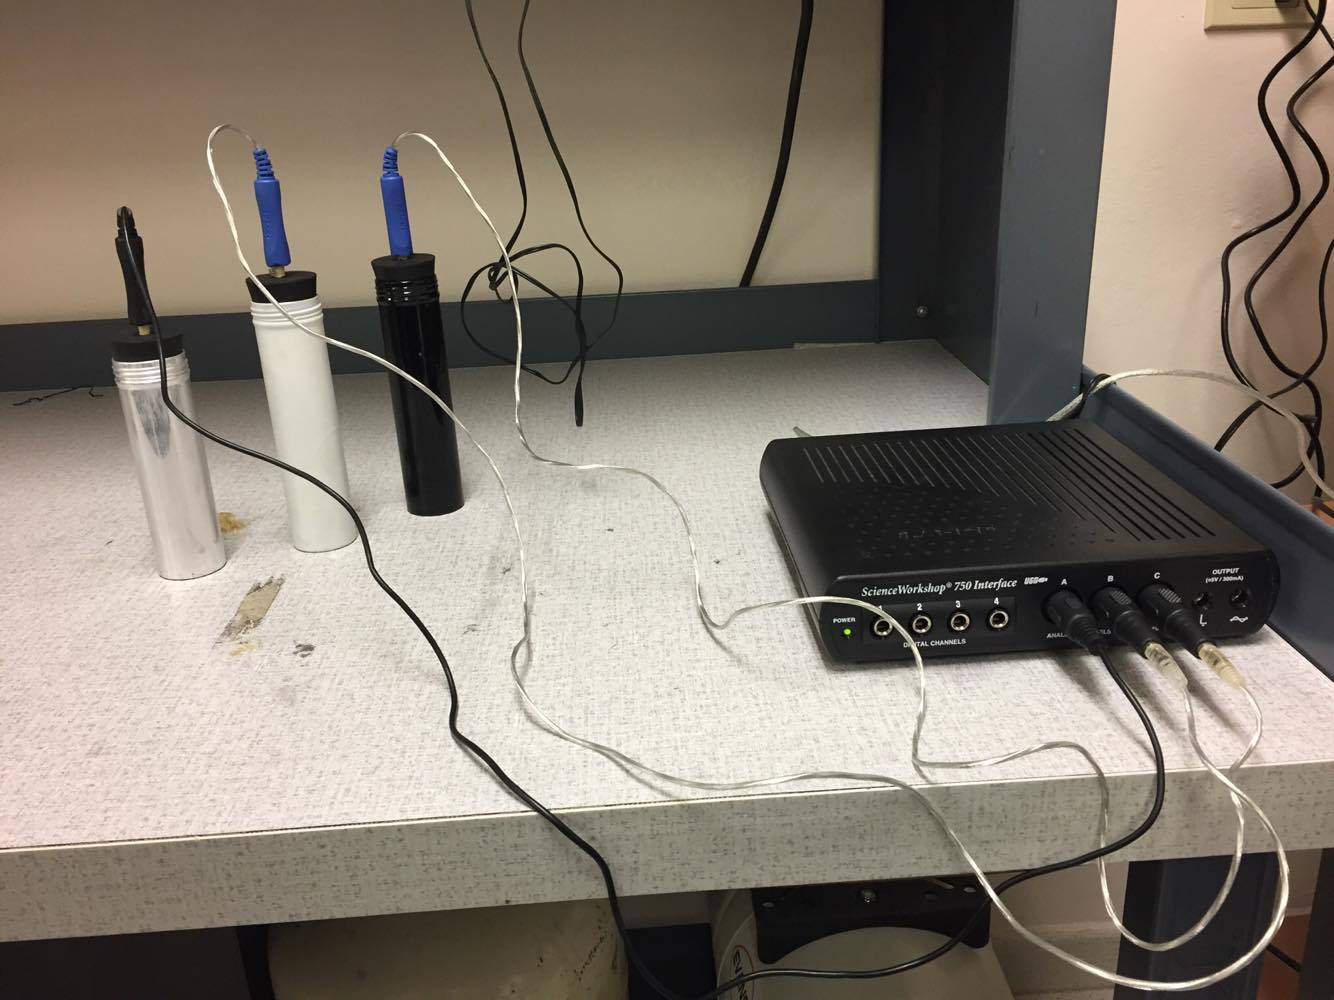
\includegraphics[height=5cm]{metal.jpg}
\caption{Arreglo del experimento con recipientes metálicos}
\end{figure}

\hspace*{0.5cm} Se conectaron los termómetro a la interfaz y se ajusto la frecuencia de muestreo a 15 segundos. El experimento duro 15 minutos. Este experimento se realizo dos veces.
\pagebreak

%===================================================================================================
\section{Resultados}
Lo que resultados que se obtuvieron se presentan en los siguientes gráficos. La figura 3 se muestra como cambia la temperatura del agua dentro de un calorímetro de exterior de metal e interior de unicel, conforme pasa el tiempo.

\begin{figure}[H]
\centering
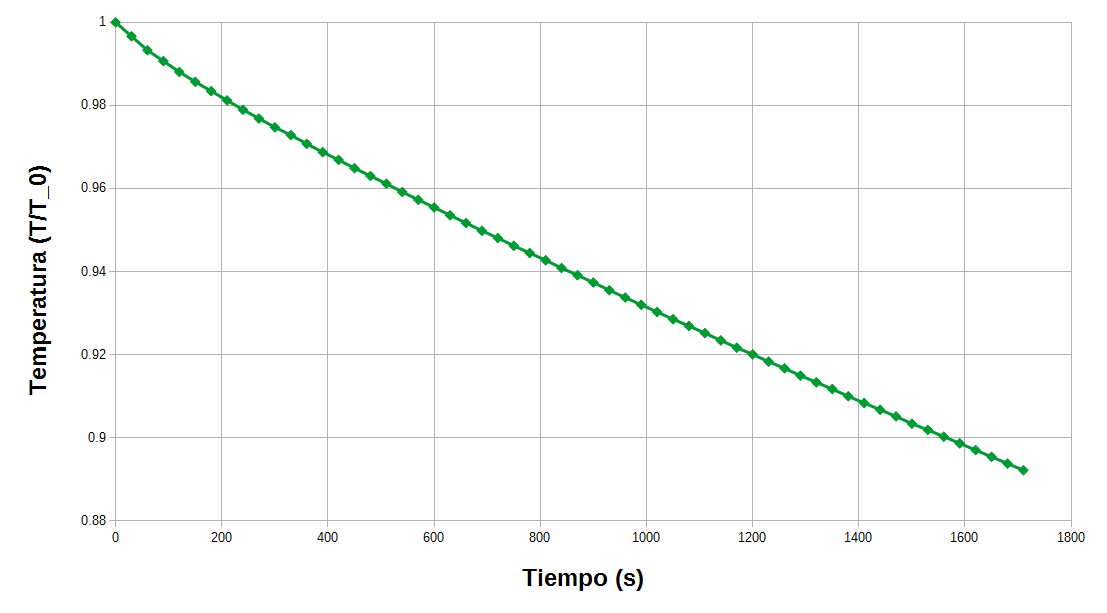
\includegraphics[scale=0.4]{GraficaCUM.png}
\caption{Variación de temperatura calorímetro de metal y unicel}
\end{figure}
La figura 4 nos muestra como cambio la temperatura del agua dentro del calorímetro de metal.
\begin{figure}[H]
\centering
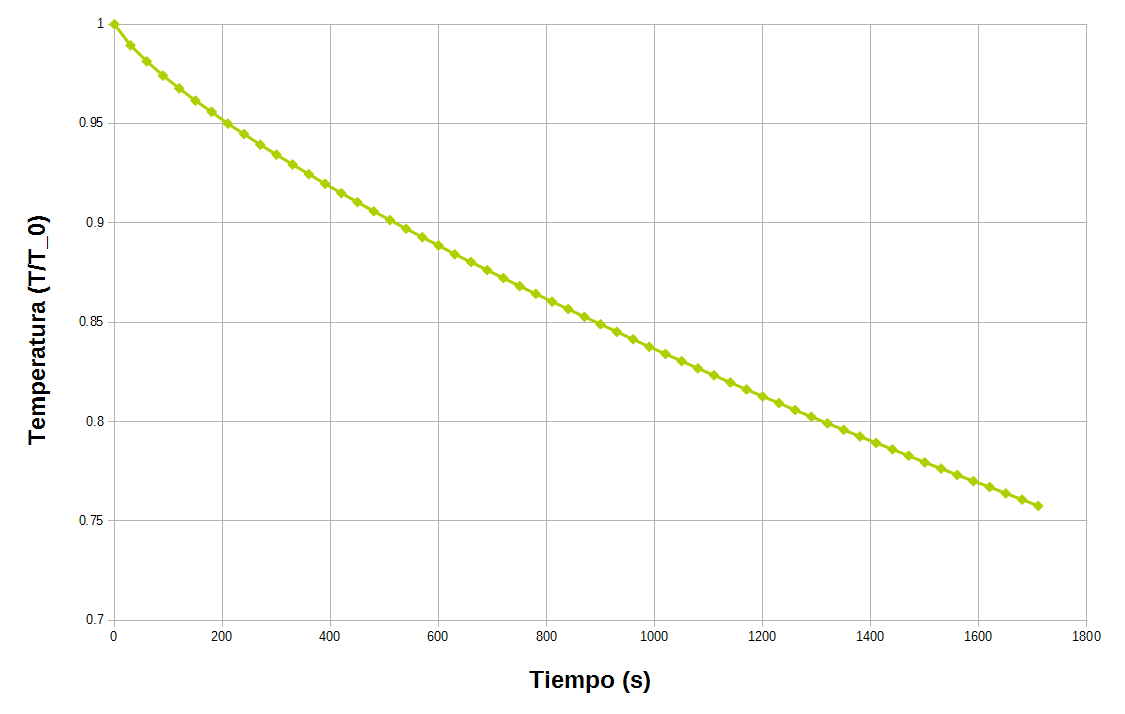
\includegraphics[scale=0.4]{GraficaCM.png}
\caption{Variación de temperatura calorímetro de metal}
\end{figure}
\pagebreak
En la figura 5 se observa como cambia la temperatura del agua en el calorímetro de unicel.

\begin{figure}[H]
\centering
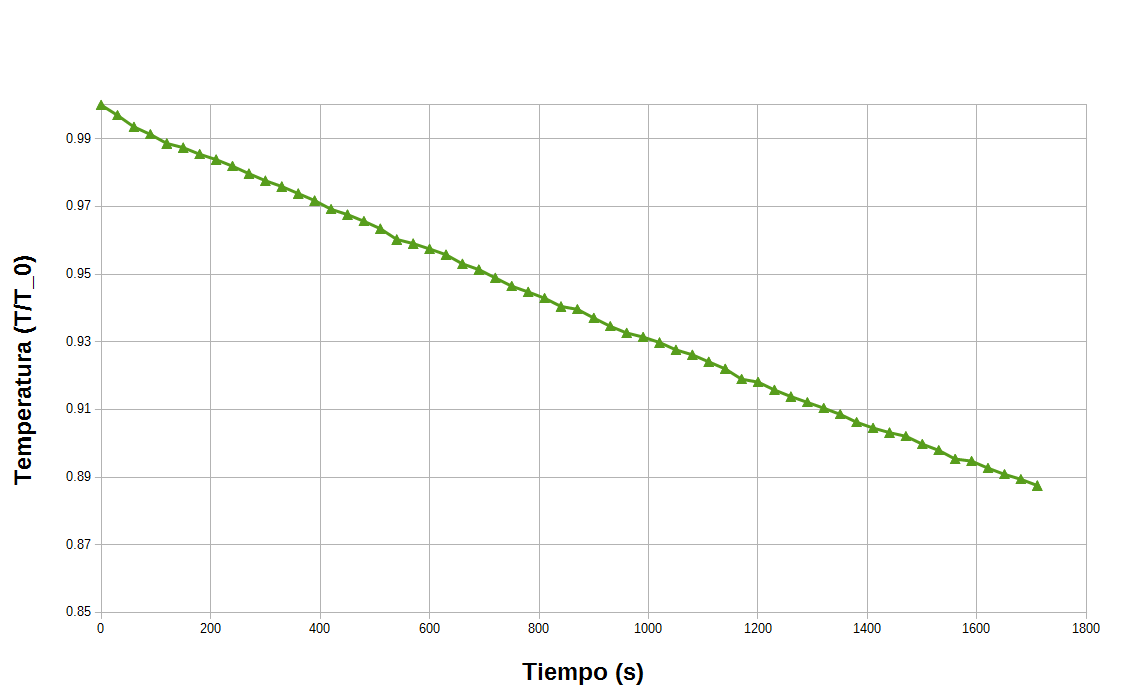
\includegraphics[scale=0.4]{GraficaCU.png}
\caption{Variación de temperatura calorímetro de unicel}
\end{figure}

Para poder obeservar cual es un mejor recipiente para mantener una condición de aislamiento adiabático, se tiene que comparar la variación de la temperatura en el mismo intervalo de tiempo.

La siguiente figura se muestra como la forma en la que varían los 3.

\begin{figure}[H]
\centering
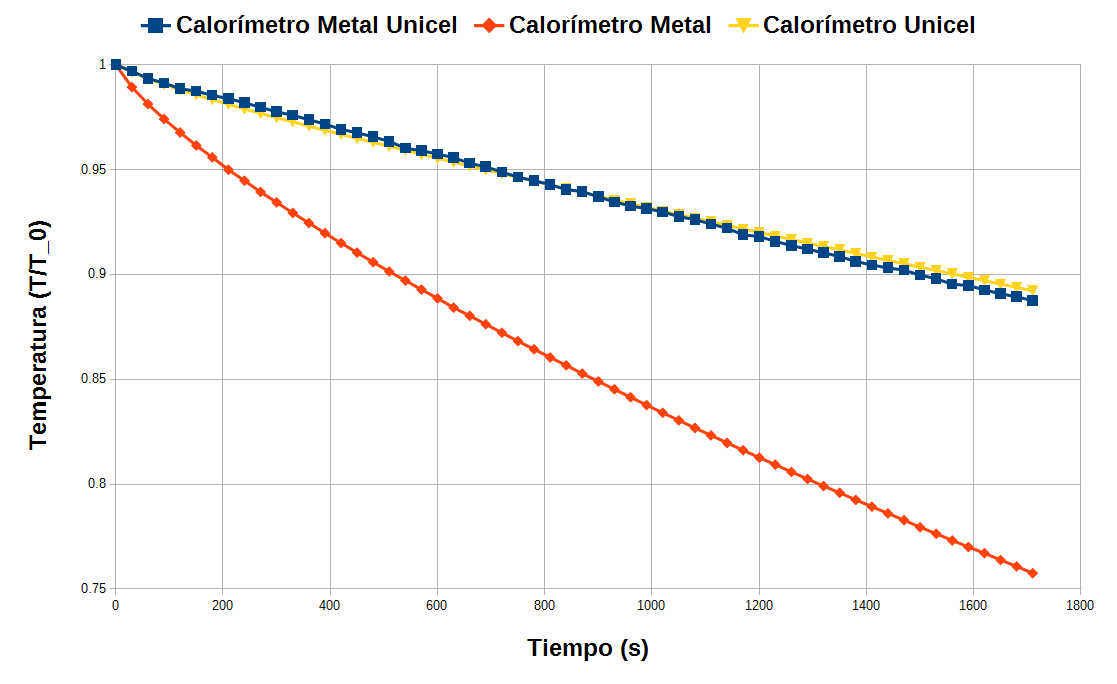
\includegraphics[scale=0.4]{GraficaC.png}
\caption{Variación de temperatura calorímetro de unicel}
\end{figure}

Como se puede observar el calorímetro de unicel y el de metal con unicel son muy buenos calorímetros para tener una condición de aislamiento adiabático. Esto se observa por como cae la temperatura en el mismo intervalo de tiempo.
\pagebreak

El segundo experimento fue observar cambia la temperatura en recipientes del mismo material y grosor pero diferente superficie exterior, en este caso el color de la superficie. Este experimento se realizaron 2 mediciones.

Los resultados obtenidos se presentan en los siguientes gráficos.
Para nuestra primera medición en el recipiente plateado, se pueden ver en la figura 7

\begin{figure}[H]
\centering
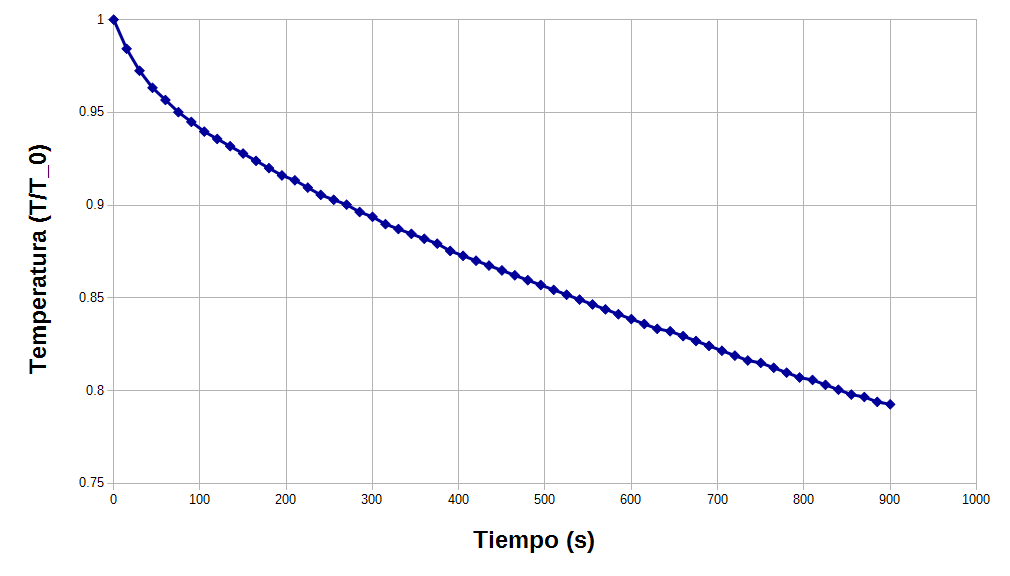
\includegraphics[scale=0.4]{CM1.png}
\caption{Medición 1 Recipiente plateado}
\end{figure}

La segunda medición se realizo con una pared de unicel entre los contenedores y se obtuvo lo que se muestra en la figura 8
\begin{figure}[H]
\centering
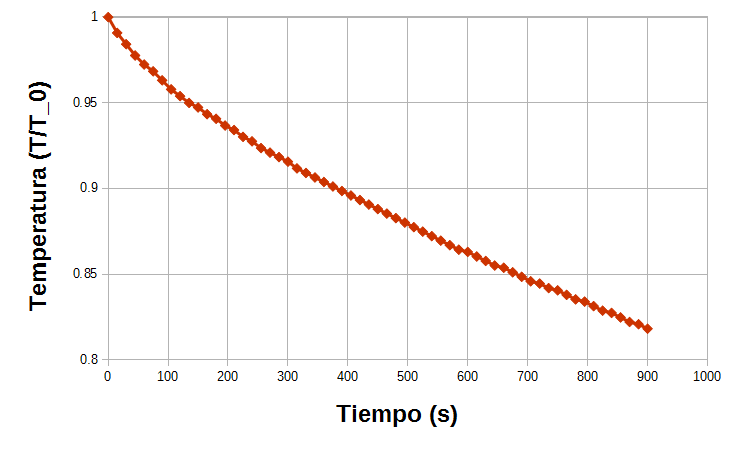
\includegraphics[scale=0.4]{CM2.png}
\caption{Medición 2 Recipiente plateado}
\end{figure}

La figura 9 muestra el efecto de la pared en la variación de la temperatura.
\begin{figure}[H]
\centering
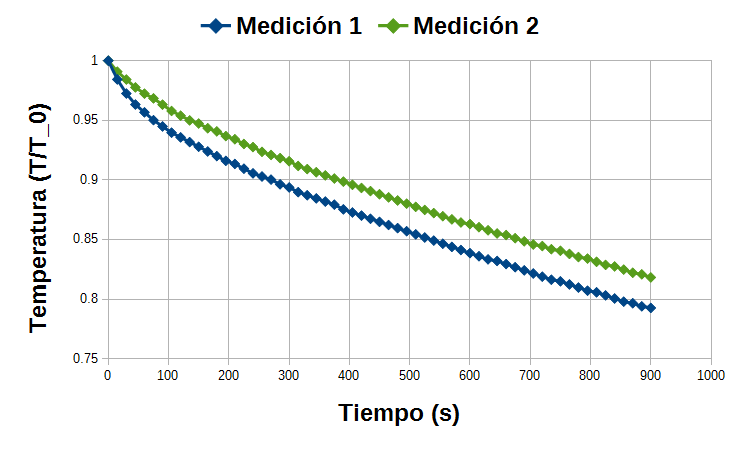
\includegraphics[scale=0.4]{CM1_2.png}
\caption{Medición 1 y 2 Recipiente plateado}
\end{figure}

Para nuestra primera medición en el recipiente blanco, se pueden ver en la figura 10

\begin{figure}[H]
\centering
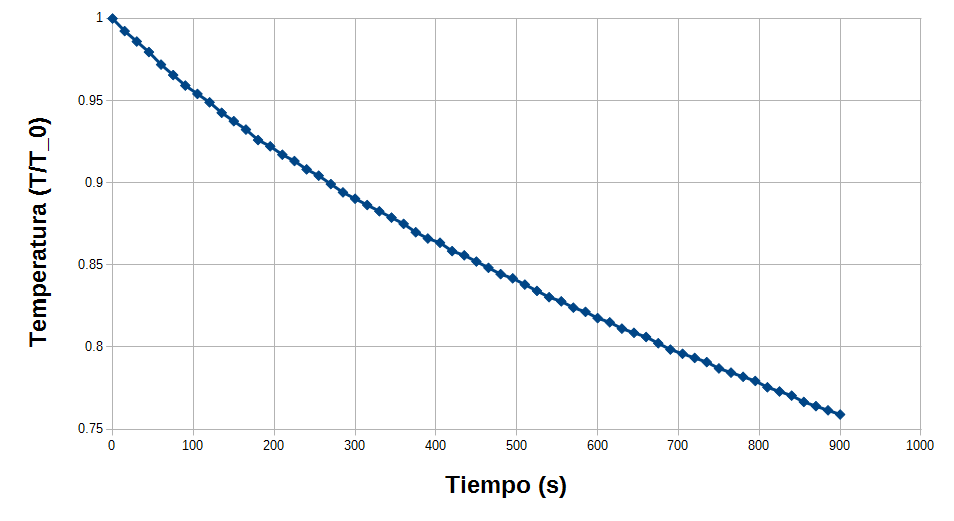
\includegraphics[scale=0.4]{CB1.png}
\caption{Medición 1 Recipiente blanco}
\end{figure}

La segunda medición se obtuvo lo que se muestra en la figura 11
\begin{figure}[H]
\centering
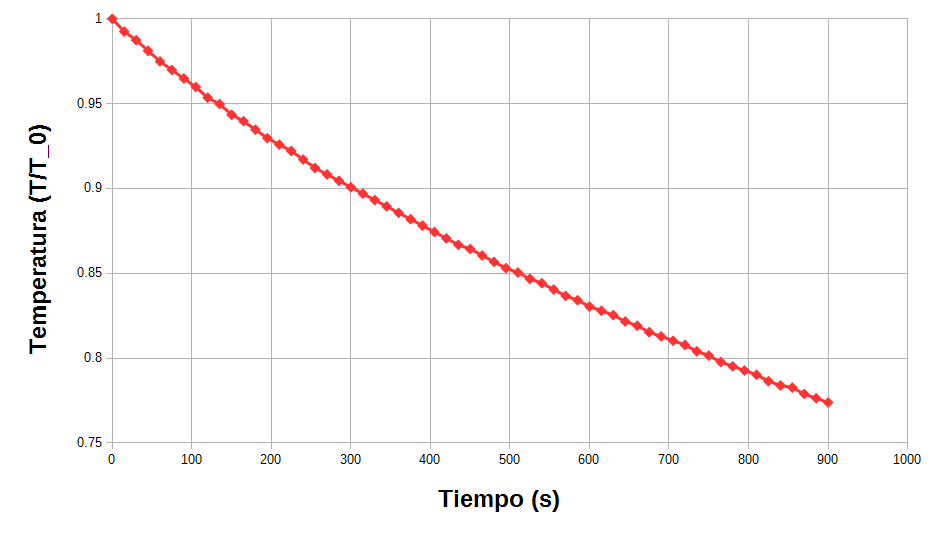
\includegraphics[scale=0.4]{CB2.png}
\caption{Medición 2 Recipiente blanco}
\end{figure}

La figura 12 muestra el efecto de la pared en la variación de la temperatura.
\begin{figure}[H]
\centering
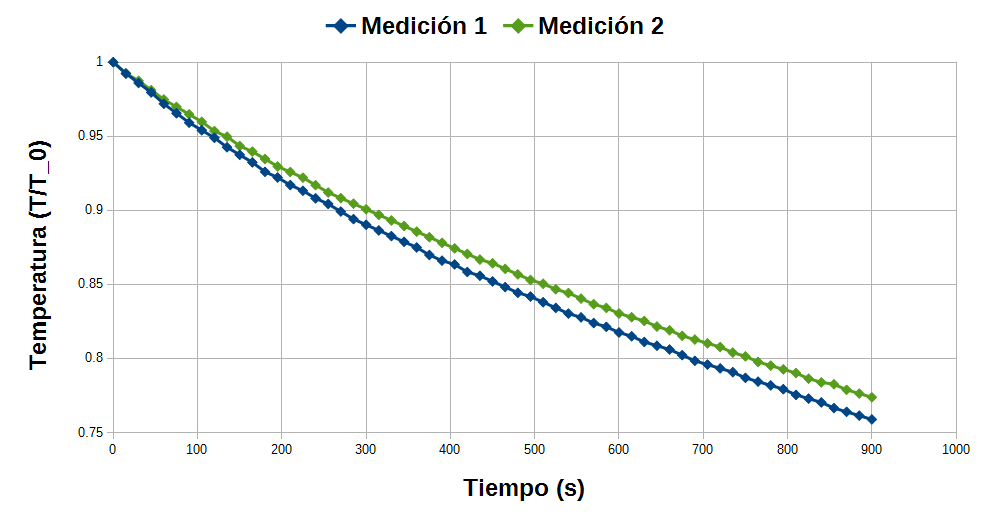
\includegraphics[scale=0.4]{CB1_2.png}
\caption{Medición 1 y 2 Recipiente blanco}
\end{figure}	

Para nuestra primera medición en el recipiente blanco, se pueden ver en la figura 13

\begin{figure}[H]
\centering
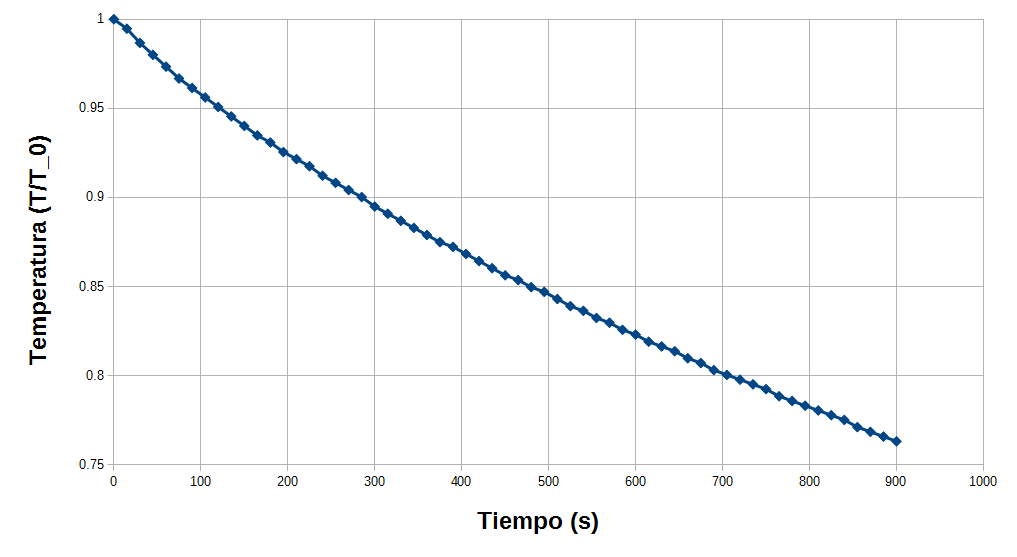
\includegraphics[scale=0.4]{CN1.png}
\caption{Medición 1 Recipiente negro}
\end{figure}

La segunda medición se obtuvo lo que se muestra en la figura 14
\begin{figure}[H]
\centering
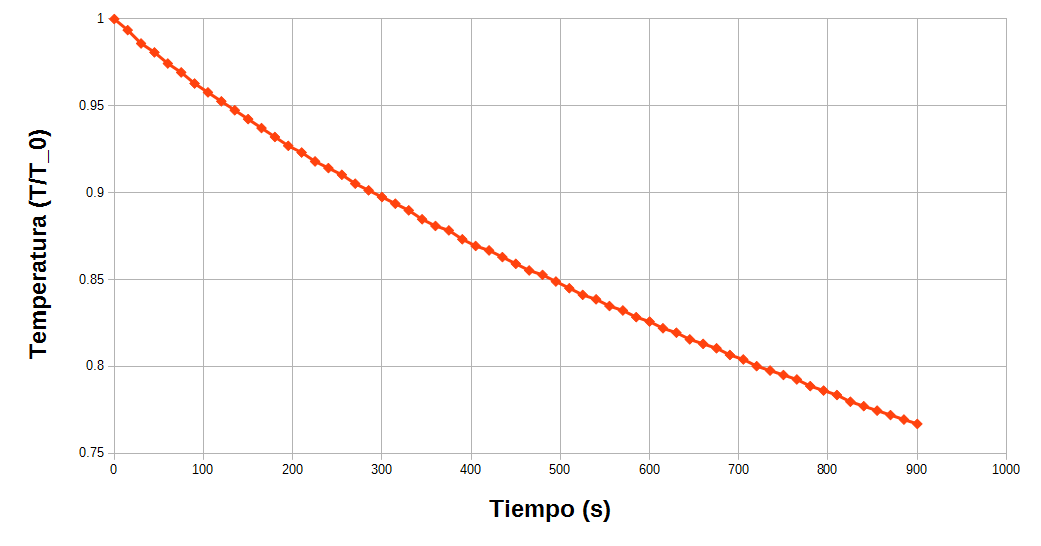
\includegraphics[scale=0.4]{CN2.png}
\caption{Medición 2 Recipiente negro}
\end{figure}

La figura 15 muestra el efecto de la pared en la variación de la temperatura.
\begin{figure}[H]
\centering
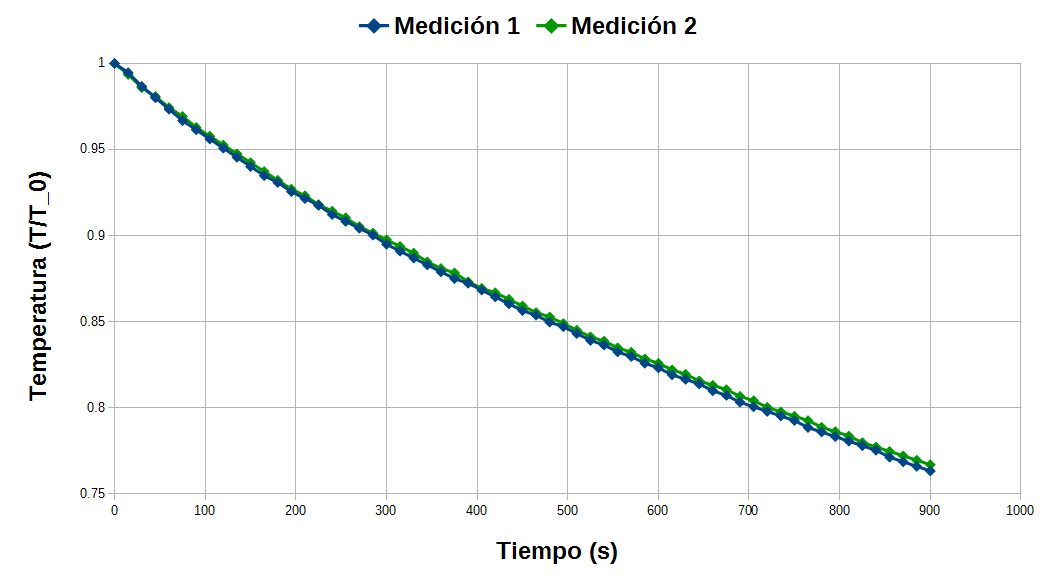
\includegraphics[scale=0.4]{CN1_2.png}
\caption{Medición 1 y 2 Recipiente negro}
\end{figure}	

La comparación entre cada recipiente en la misma medición fue la siguiente. La figura 16 es de la primera medición.

\begin{figure}[H]
\centering
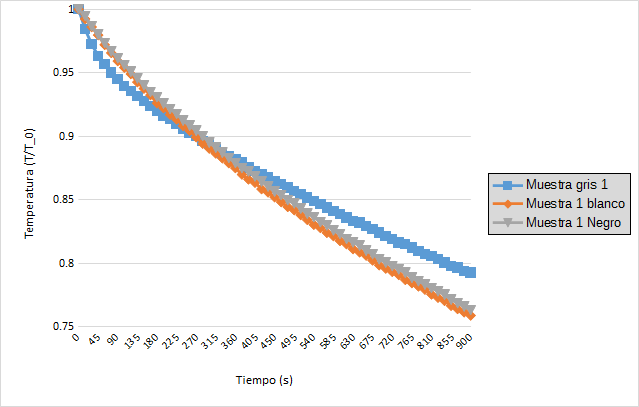
\includegraphics[scale=0.75]{med1.png}
\caption{Comparación de la medición 1}
\end{figure}	
\pagebreak
La figura 17 muestra el de la segunda medición
\begin{figure}[H]
\centering
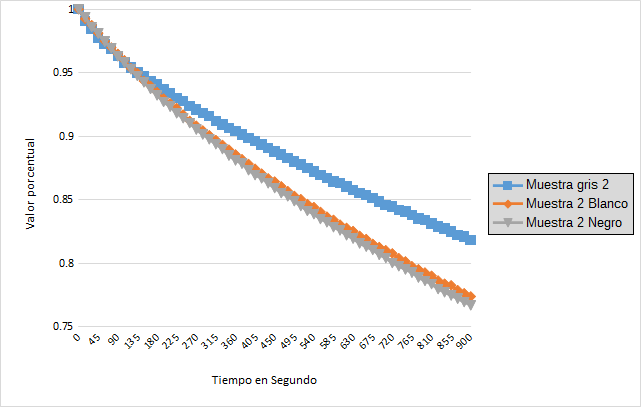
\includegraphics[scale=0.75]{med2.png}
\caption{Comparación de la medición 1}
\end{figure}

En la primera medición, el gris fue el que menos disminuyo su temperatura y el blanco el mas. Lo mismo se observa con la segunda medición. También se ve que en la segunda medición las temperaturas disminuyen menos que en la segunda. El recipiente negro en las dos mediciones tiene una disminución en la temperatura similar.
\vspace{-.5cm}
%===================================================================================================
\section{Discusión}
En esta practica se realizaron dos experimentos. En el primero se esperaba observar que uno de los recipientes iba a ser mejor candidato para mantener una condición de aislamiento adiabático. Como se esperaba, los recipientes con unicel mantienen mejor esta condición.

En el segundo experimento, se observo si el color de la superficie influenciaba la forma en que cambia la temperatura. El experimento nos muestra que el color si afecta al cambio de la temperatura. Esto si se esperaba, pero lo que no es que los que estuvieran pintados de blanco y negro tuvieran un variación tan parecida.
\vspace{-.5cm}
%===================================================================================================
\section{Conclusiones}
Se puede concluir en el primer experimento que de hecho, el material afecta la forma en la que varia la temperatura de su contenido. Lo que se observa es que el unicel es el mejor de los materiales para mantener una condición de aislamiento adiabático. En el segundo experimento se concluyo que la superficie es un factor a la hora de mantener la temperatura.

\pagebreak
%================================================================================================
\section{Apéndice}
Las tablas de las mediciones se pueden encontrar en la siguiente vinculo.
\url{https://drive.google.com/file/d/0B3misvJiB_DQLWw3VE45YVYwa00/view?usp=sharing}

\begin{thebibliography}{6}

	
\bibitem{termopasco}
	\textit{Quad Temperature Sensor PS -2143}. Recuperado de   \url{http://www.pasco.com}

\bibitem{termo} 
\textit{PASPORT-Temperature-Sensor-Manual-PS-2125} Recuperado de  \url{http://www.pasco.com}

\bibitem{acu}
Acu\~na, H. (2015). \textit{Manual de Guías de Experiencias en el Laboratorio de Termodinámica Clásica}.

\end{thebibliography}
%================================================================================================

\end{document}

